\myparagraph{
    \begin{tcolorbox}[colback=blue!5!white, colframe=blue!75!black]
        Il pattern permette di assegnare a ogni record di tabella e a ogni oggetto un
        valore alfanumerico chiamato Object ID che consente l'immediata identificazione
        di ogni istanza.
    \end{tcolorbox}

    \begin{center}
        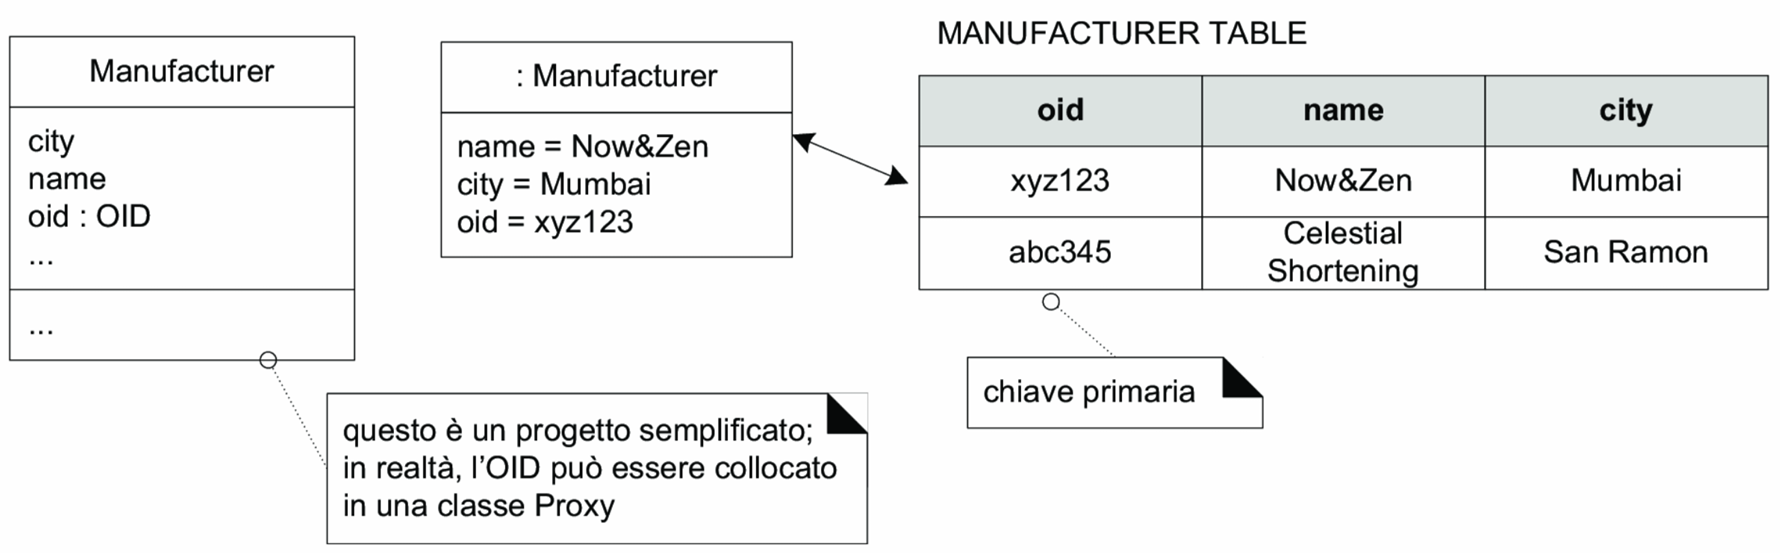
\includegraphics[scale=0.25]{Esercitazione - Design Patterns/Object Identifier.png}
    \end{center}
}